% !TEX root = ../main.tex
%-------------------------------------------------------------------------------
%-------------------------------------------------------------------------------
\begin{frame}\begin{center}
		\LARGE\textbf{Parallel processing}
\end{center}\end{frame}
%-------------------------------------------------------------------------------
%-------------------------------------------------------------------------------
\begin{frame}\textbf{Memory access}\vspace{0.3cm}

\begin{itemize}\setlength\itemsep{1em}
    \item shared memory
    \item distributed memory
\end{itemize}

\end{frame}
%-------------------------------------------------------------------------------
%-------------------------------------------------------------------------------
\begin{frame}
  	\begin{figure}[htp]\centering
      \scalebox{0.3}{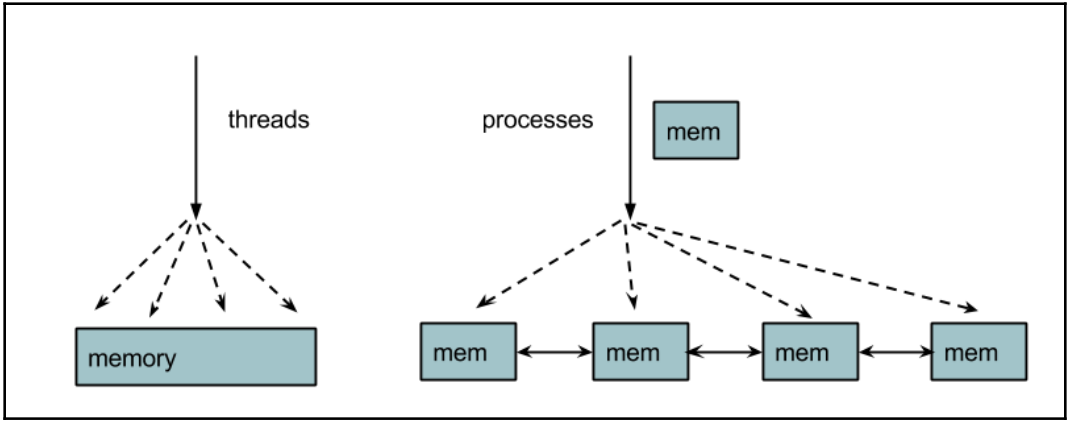
\includegraphics{fig-memory-access}}
  	\end{figure}
\end{frame}
%-------------------------------------------------------------------------------
%-------------------------------------------------------------------------------
\begin{frame}\textbf{Multiprocessing}\vspace{0.3cm}

\begin{itemize}\setlength\itemsep{1em}
    \item Let's explore the multiprocessing module in a notebook.\end{itemize}

\end{frame}
%-------------------------------------------------------------------------------
%-------------------------------------------------------------------------------
